\documentclass[11pt,a4paper]{article}

\usepackage[margin=2.1cm]{geometry}
\usepackage{graphicx}
\usepackage{xcolor}
\usepackage{listings}

\setlength{\parindent}{0pt}
\lstset{
    language=Python,
    basicstyle=\ttfamily\small,
    keywordstyle=\color{blue!55!black},
    commentstyle=\color{gray!70!black},
    stringstyle=\color{teal!55!black},
    columns=fullflexible,
    keepspaces=true,
    showstringspaces=false,
    breaklines=true,
    frame=single,
    rulecolor=\color{black!25},
    framesep=5pt
}

\begin{document}

\begin{center}
    {\LARGE\bfseries Programming Assignment\par}
    \vspace{0.2em}
    {\Large\bfseries Estimating $\pi$ Using Monte Carlo Simulation\par}
    \vspace{0.45em}
    {\large Course: Probability and Mathematical Statistics\par}
\end{center}
\vspace{0.3em}
\noindent\rule{\textwidth}{0.4pt}

\section{Python Source Code}
\lstinputlisting{SI140A_HW_1.py}

\clearpage
\section{Error Curve}
\begin{center}
    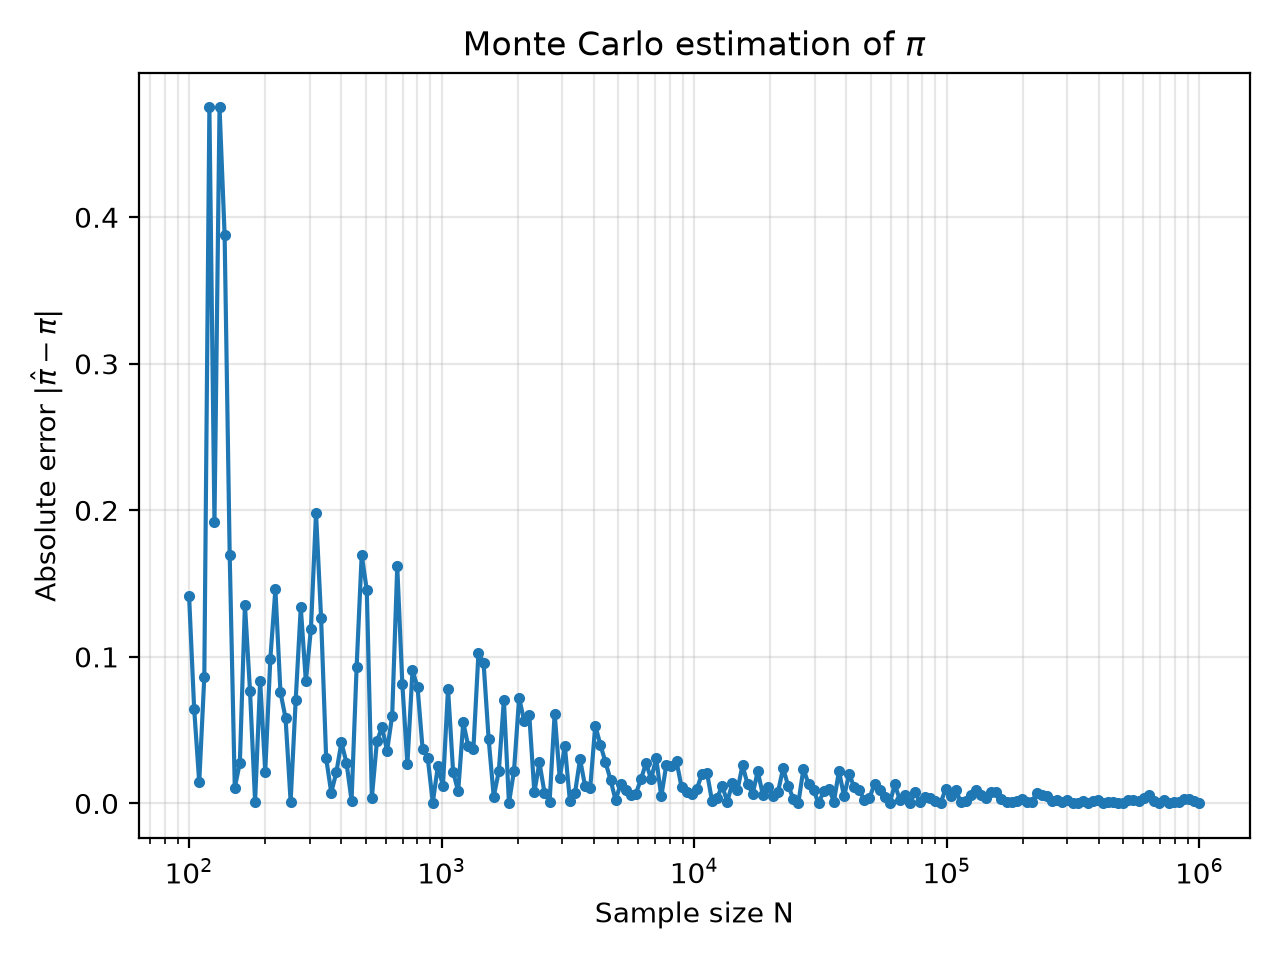
\includegraphics[width=0.92\textwidth]{error_curve.png}
\end{center}

\end{document}
